
%------------------ Präambel ---------------------------------------------------
\documentclass[envcountsame, envcountchap, deutsch]{i-studis}

\usepackage[utf8]{inputenc}

\usepackage[a4paper]{geometry}
\usepackage[english, ngerman]{babel}

\usepackage[pdftex]{graphicx}
\usepackage{epstopdf}

% Zeilenabstand auf 1.5 setzen
\renewcommand{\baselinestretch}{1.5}

\usepackage{listings}

\usepackage[german, ruled, vlined]{algorithm2e}
\usepackage{amssymb, amsfonts, amstext, amsmath}
\usepackage{array}
\usepackage[skip=10pt]{caption}
\usepackage[usenames, dvipsnames]{color}
\usepackage[pdftex, plainpages=false]{hyperref}
\usepackage{textcomp}

\usepackage{bibgerm}
\bibliographystyle{geralpha}

\usepackage{makeidx}
\usepackage{multicol}
\usepackage{float}
\makeindex

\pagestyle{myheadings}
\setlength{\textheight}{1.1\textheight}
\setlength{\parindent}{0pt}
\setlength{\parskip}{6pt} % Beispiel für 6pt Abstand zwischen Absätzen
\lstset{
	basicstyle=\scriptsize\ttfamily,
	commentstyle=\scriptsize\ttfamily\color{Gray},
	identifierstyle=\scriptsize\ttfamily,
	keywordstyle=\scriptsize\ttfamily,
	stringstyle=\scriptsize\ttfamily,
	tabsize=4,
	numbers=left,
	numberstyle=\tiny,
	numberblanklines=false,
	frame=single,
	framesep=3mm,
	framexleftmargin=7mm,
	xleftmargin=10mm,
	linewidth=144mm,
	captionpos=b,
}

%------------------ Manuelle Silbentrennung ------------------------------------
\hyphenation{Ele-men-tar-ob-jek-te ab-ge-tas-tet Aus-wer-tung House-holder-Matrix Least-Squares-Al-go-ri-th-men}


%------------------ Titelseite -------------------------------------------------
\begin{document}

\title{Rubiks Cube Dokumentation}
%\subtitle{English Title of the Thesis}

\author{Florian Wößner}

\supervisor{Prof. Dr. Christoph Lürig}

\address{Trier}
\submitdate{02.02.2025}

%------------------ Projektart -------------------------------------------------
%\project{Bachelor-Projektarbeit}
%\project{Bachelor-Abschlussarbeit}
%\project{Master-Projektstudium}
%\project{Master-Abschlussarbeit}
%\project{Seminar}
\project{Hausarbeit}

\mytitlepage

%------------------ Vorwort, Kurzfassung, Verzeichnisse ------------------------
\frontmatter
%\preface

Ein Vorwort ist nicht unbedingt nötig. Falls Sie ein Vorwort schreiben, so ist dies der Platz, um z.B. die Firma vorzustellen, in der diese Arbeit entstanden ist, oder um den Personen zu danken, die in irgendeiner Form positiv zur Entstehung dieser Arbeit beigetragen haben.

Auf keinen Fall sollten Sie im Vorwort die Aufgabenstellung näher erläutern oder vertieft auf technische Sachverhalte eingehen.
								% Vorwort (optional)
%\kurzfassung

In der Kurzfassung soll in kurzer und prägnanter Weise der wesentliche Inhalt der Arbeit beschrieben werden. Dazu zählen vor allem eine kurze Aufgabenbeschreibung, der Lösungsansatz sowie die wesentlichen Ergebnisse der Arbeit. Ein häufiger Fehler für die Kurzfassung ist, dass lediglich die Aufgabenbeschreibung (d.h. das Problem) in Kurzform vorgelegt wird. Die Kurzfassung soll aber die gesamte Arbeit widerspiegeln. Deshalb sind vor allem die erzielten Ergebnisse darzustellen. Die Kurzfassung soll etwa eine halbe bis ganze DIN-A4-Seite umfassen.

Hinweis: Schreiben Sie die Kurzfassung am Ende der Arbeit, denn eventuell ist Ihnen beim Schreiben erst vollends klar geworden, was das Wesentliche der Arbeit ist bzw. welche Schwerpunkte Sie bei der Arbeit gesetzt haben. Andernfalls laufen Sie Gefahr, dass die Kurzfassung nicht zum Rest der Arbeit passt.

\kurzfassungEN

The same in English.
							% Kurzfassung/Abstract
\tableofcontents										% Inhaltsverzeichnis
%\listoffigures											% Abbildungsverzeichnis (optional)
%\listoftables											% Tabellenverzeichnis (optional)
%\lstlistoflistings										% Listings (optional)


%------------------ Kapitel ----------------------------------------------------
\mainmatter
\chapter{Einleitung}
Das Rubik’s Cube Projekt wurde im Rahmen des Moduls Spieleprogrammierung - Vertiefung entwickelt. Ziel des Projekts war es, einen interaktiven Rubik’s Cube zu simulieren, der mithilfe von Maus- und Tastatureingaben gesteuert werden kann. Die technische Umsetzung erfolgte unter Verwendung von C++ und OpenGL, wobei mathematische Konzepte wie Quaternionen und Transformationen zur Anwendung kamen.

In dieser Hausarbeit werden die Funktionsweisen der wichtigsten Klassen und die grundlegenden Lösungsideen dokumentiert. Der Fokus liegt auf den entwickelten Ansätzen sowie einer oberflächlichen Beschreibung der Implementierung.

\section{Steuerung}
Der Rubik’s Cube wird vollständig durch Maus- und Tastatureingaben gesteuert:

\begin{itemize}
    \item Rechte Maustaste gedrückt: Durch Ziehen wird der gesamte Cube rotiert.
    \item Linke Maustaste gedrückt: Ermöglicht das Drehen einzelner Slices (Zeilen und Spalten).
    \item Leertaste: Setzt den Würfel in den Ausgangszustand zurück.
    \item Scrollrad: Kann benutzt werden, um mit der Kamera herein- oder herauszuzoomen.
\end{itemize}

\chapter{Umsetzung}
In diesem Kapitel werden die wichtigsten Klassen und deren Funktionsweisen erläutert. Jede Klasse wird kurz beschrieben, wobei der Fokus auf ihrer Rolle im Gesamtsystem und ihrer Implementierung liegt.

\section{Klassenübersicht}
Das Klassendiagramm zeigt die Beziehungen der wichtigsten Komponenten des Rubik's Cube Projekts. Die Basis bildet das Interface \texttt{IGameInterface}, das von \texttt{RubiksGameInterface} implementiert wird. Diese zentrale Klasse koordiniert das Zusammenspiel von Eingaben (\texttt{InputSystem}, unterstützt durch \texttt{KeyboardObserver}), der Logik (\texttt{RubiksCube}) und der Darstellung (\texttt{CubieRenderer}).

Der Würfel selbst besteht aus \texttt{Cubie}-Objekten, die von \texttt{RubiksCube} organisiert werden. Zur Unterstützung von Rendering-Aufgaben wird die Klasse \texttt{ShaderUtil} genutzt, welche die Shader-Verwaltung übernimmt. Abbildung \ref{SimpleClassDia} verdeutlicht die Beziehungen der Klassen.

\begin{figure} [H]
	\centering
	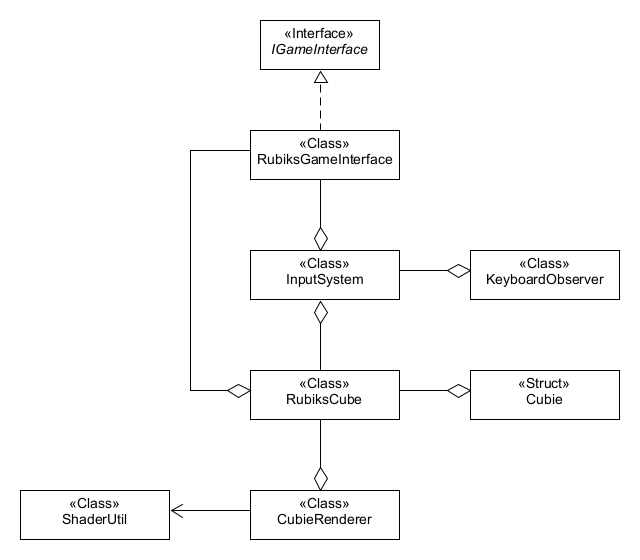
\includegraphics[scale=0.6]{images/SimpleClassDia.png}
	\caption{Vereinfachtes Klassendiagramm}
	\label{SimpleClassDia}
\end{figure}

\section{main.cpp}
Der Code in \texttt{main.cpp} dient als Einstiegspunkt des Projekts. Hier wird \textit{GLFW} initialisiert, ein Fenster erstellt und die \textit{GLEW}-Bibliothek geladen, um moderne OpenGL-Funktionen nutzen zu können. Ein \texttt{RubiksGameInterface}-Objekt wird erstellt und als aktuelle Schnittstelle festgelegt. Der Game-Loop verarbeitet Benutzereingaben und rendert das Fenster. Ein zusätzlicher Mechanismus stellt sicher, dass das Programm bei minimiertem Fenster nicht abstürzt. Nach dem Schließen des Fensters werden mit der Methode \texttt{ShutdownSystem()} alle Ressourcen freigegeben und \textit{GLFW} ordnungsgemäß beendet.


\section{RubiksGameInterface und IGameInterface}
Die Klasse \texttt{RubiksGameInterface} implementiert das Interface \texttt{IGameInterface} und stellt die zentrale Schnittstelle für die Verwaltung des Spiels dar.
Die Methode \texttt{Initialize(GLFWwindow* window)} kümmert sich um die Initialisierung des Spielfensters und des Eingabesystems. Dabei wird das Fensterobjekt in \texttt{m\_window} gespeichert und das Eingabesystem durch den Aufruf von \texttt{m\_input.Initialize(window)} eingerichtet. Der Rubik's Cube wird durch \texttt{m\_rubiksCube.Initialize(*this)} initialisiert. Zusätzlich wird mit \texttt{m\_input.ObserverKey(GLFW\_KEY\_SPACE)} ein Observer für die Leertaste erstellt.

Die Methode \texttt{Render(float aspectRatio)} ist für das Zeichnen des Fensters und des Rubik's Cube verantwortlich. Sie berechnet bei Bedarf die Projektions- und View-Matrizen neu, wenn die Kameraposition oder das Seitenverhältnis des Fensters sich geändert haben. Anschließend wird die Renderlogik auf den Rubik's Cube angewendet, um dessen aktuellen Zustand mit dem Aufruf von \texttt{m\_rubiksCube.Render(m\_projection * m\_view)} darzustellen.

Die Methode \texttt{Update(double deltaTime)} verarbeitet die Benutzereingaben und aktualisiert den Rubik's Cube. Wenn die Leertaste gedrückt wird, erfolgt ein Zurücksetzen des Rubik's Cubes, andernfalls wird \texttt{m\_rubiksCube.Update(*this)} aufgerufen. Änderungen der Kameraentfernung, die durch das Mausrad bedingt sind, werden in Echtzeit aktualisiert, indem der Wert von \texttt{m\_CameraDistance} angepasst wird. Der Kameraabstand wird durch \texttt{if}-Abfragen auf bestimmte Werte begrenzt. Die Methode \texttt{ClearResources()} gibt die Ressourcen des \texttt{m\_rubiksCube}-Objektes frei.

Zusätzlich verfügt die Klasse über die Methode \texttt{QueueMatrixRecalculation()}, die es ermöglicht, das Neuberechnen der Projektions- und View-Matrizen gezielt anzustoßen.
Weitere Getter-Methoden erlauben den Zugriff auf \texttt{m\_deltaTime} und \texttt{m\_input}. 

Abbildung \ref{RubiksGameInterfaceDia} zeigt das Klassendiagramm zu diesem Abschnitt.

\begin{figure} [H]
	\centering
	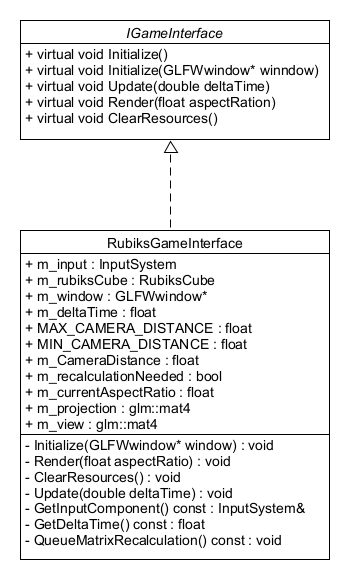
\includegraphics[scale=0.6]{images/GameInterfaceClassDia.png}
	\caption{Klassendiagramm RubiksGameInterface}
	\label{RubiksGameInterfaceDia}
\end{figure}

\section{InputSystem und KeyboardObserver}
Die Klasse \texttt{InputSystem} ist eine zentrale Komponente zur Verwaltung von Benutzereingaben, die sowohl Maus- als auch Tastatureingaben verarbeitet.

Ein zentrales Merkmal des \texttt{InputSystem} ist die Verwaltung der Maustasten-Zustände. Diese werden durch die Enumeration \texttt{ClickState} repräsentiert, die die Zustände \texttt{NO\_ACTION}, \texttt{CLICK}, \texttt{HOLD} und \texttt{RELEASE} definiert. Diese Zustände werden in den Membern \texttt{m\_leftClickState} und \texttt{m\_rightClickState} gespeichert und können über die Methoden \texttt{GetLeftClickState()} und \texttt{GetRightClickState()} abgefragt werden. Dadurch müssen sich andere Klassen nicht um die Details der Zustandsverwaltung kümmern. Zusätzlich wird der aktive Maustasten-Zustand durch die Enumeration \texttt{MouseButton} verwaltet, die die möglichen Maustasten wie \texttt{LEFT\_BUTTON}, \texttt{RIGHT\_BUTTON} und \texttt{NO\_BUTTON} definiert.

Die Aktualisierung der Maustasten-Zustände erfolgt in der \texttt{Update()}-Methode, die regelmäßig aufgerufen wird. Die Methode \texttt{UpdateClickState(MouseButton mouseButton, ClickState\& clickState)} wird dabei verwendet, um den Zustand einer Maustaste basierend auf den aktuellen \textit{GLFW}-Eingaben zu aktualisieren. Dabei wird auch die aktive Maustaste berücksichtigt, um sicherzustellen, dass nicht beide Maustasten gleichzeitig aktiv sind.

Mit den Methoden \texttt{ScreenToWorld(const glm::vec2\& screenPosition)} und \texttt{WorldToScreen(const glm::vec2\& screenPosition)} gibt es auch Möglichkeiten zur Umrechnung zwischen Bildschirmkoordinaten und Weltkoordinaten. Zusätzlich kann mit der Methode \texttt{GetPickingRay(glm::vec3\& out\_origin, glm::vec3\& out\_direction)} ein Strahl erzeugt werden, der in die Richtung der aktuellen Mausposition in die Szene zeigt, um Interaktionen wie das Ziehen von Objekten zu unterstützen.

Die Behandlung des Mausrads erfolgt über eine statische Callback-Funktion \\\texttt{ScrollCallback(GLFWwindow* window, double xScroll, double yScroll)}, \\die von \textit{GLFW} aufgerufen wird, wenn der Benutzer das Mausrad bewegt. Der Scroll-Offset wird in dem statischen Member \texttt{m\_mouseScrollOffset} gespeichert und kann über die Methode \texttt{GetMouseWheelScrollOffset()} abgerufen werden. 

Für die Tastatureingabe wird eine Map von \texttt{KeyboardObserver}-Objekten verwendet, die jeweils den Zustand einer bestimmten Taste verwalten. Der Zustand einer Taste kann über die Methoden \texttt{WasKeyDown(int key)}, \texttt{WasKeyPressed(int key)} und \texttt{WasKeyReleased(int key)} abgefragt werden Die Klasse \texttt{KeyboardObserver} speichert den Zustand einer Taste in den Membern \texttt{m\_wasDown}, \texttt{m\_wasPressed} und \texttt{m\_wasReleased}, die in der \texttt{Update()}-Methode der \texttt{KeyboardObserver}-Klasse aktualisiert werden. 

Eine detaillierte Übersicht der Klassenstruktur ist in Abbildung \ref{InputSystemDia} dargestellt.

\begin{figure} [H]
	\centering
	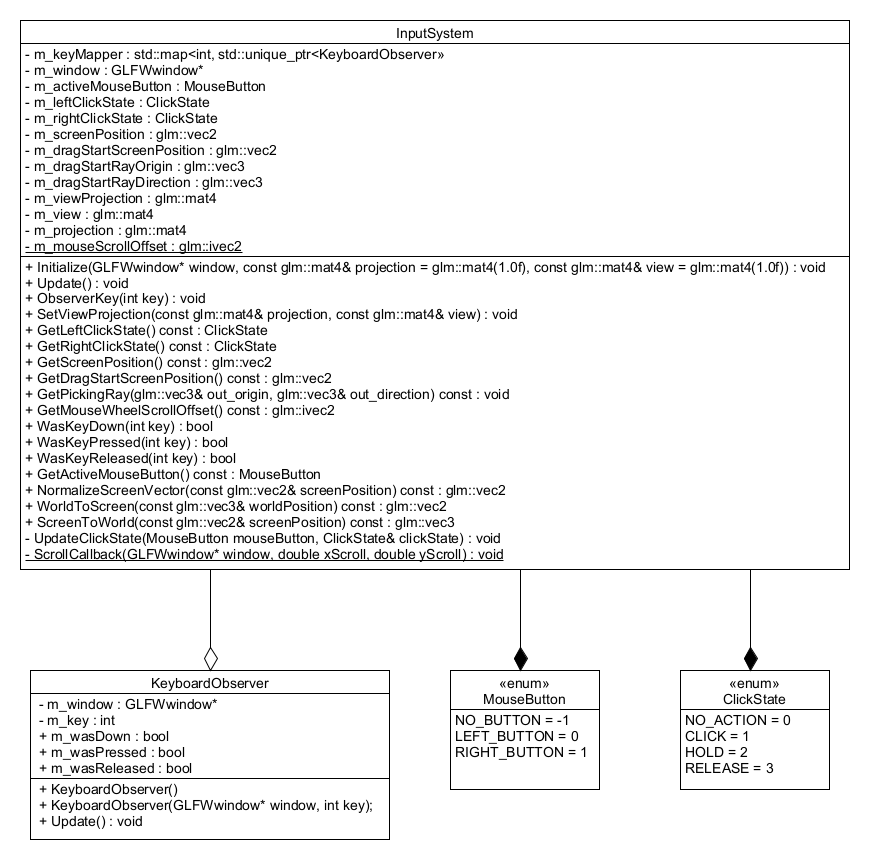
\includegraphics[scale=0.475]{images/InputSystemClassDia.png}
	\caption{Klassendiagramm InputSystem und KeyboardObserver}
	\label{InputSystemDia}
\end{figure}
\newpage
\section{CubieRenderer und ShaderUtil}
Die Klasse \texttt{CubieRenderer} ist für das Rendern der einzelnen Cubies eines Rubik's Cube zuständig. Sie verwaltet die OpenGL-Ressourcen wie Vertex-Buffer, Shader und Texturen, die für die Darstellung der Cubies benötigt werden. Die Initialisierung der Render-Ressourcen erfolgt in der Methode \texttt{Initialize()}, die die Vertex-Daten für die Positionen, Farben und Texturkoordinaten der Cubie-Seiten generiert und in OpenGL-Buffern speichert. Zusätzlich wird ein Shader-Programm geladen, das für die Transformation und das Texturieren der Cubies verantwortlich ist.

Die Methode \texttt{Render(const glm::mat4\& viewProjection, const glm::mat4\& model)} zeichnet einen einzelnen Cubie unter Verwendung der übergebenen Transformationsmatrizen. Die Cubies bestehen aus 36 Vertices, die die sechs Seiten des Würfels repräsentieren. Eine Seite besteht also aus 6 Vertices (zwei Dreiecke). Die Textur wird aktiviert und gebunden, um die Oberfläche der Cubies zu gestalten. Nach dem Rendern werden die OpenGL-Ressourcen wieder freigegeben, um Konflikte mit anderen Render-Operationen zu vermeiden.

Die Klasse \texttt{ShaderUtil} bietet Hilfsfunktionen für das Laden und Kompilieren von Shadern sowie das Laden von Texturen. Dazu gehört \texttt{CreateShaderProgram(const char* vertexFilename, const char* fragmentFilename)}, diese Methode lädt mit \texttt{LoadFile(const char* fileName)} die Vertex- und Fragment-Shader aus Dateien, kompiliert sie und verknüpft sie zu einem Shader-Programm. Dabei auftretende Fehler werden durch die Methoden \texttt{PrintShaderLog(GLuint shader)} und \texttt{PrintProgramLog(GLuint shader)} protokolliert. 

Mit \texttt{LoadTexture(const char* textureFilename)} wird eine 2D-Textur aus einer Bilddatei geladen und die Texturparameter für das Rendering konfiguriert.

Die Struktur und die Beziehungen der Klassen \texttt{CubieRenderer} und \texttt{ShaderUtil} sind detailliert in Abbildung \ref{CubieRendererDia} dargestellt.

\begin{figure} [H]
	\centering
	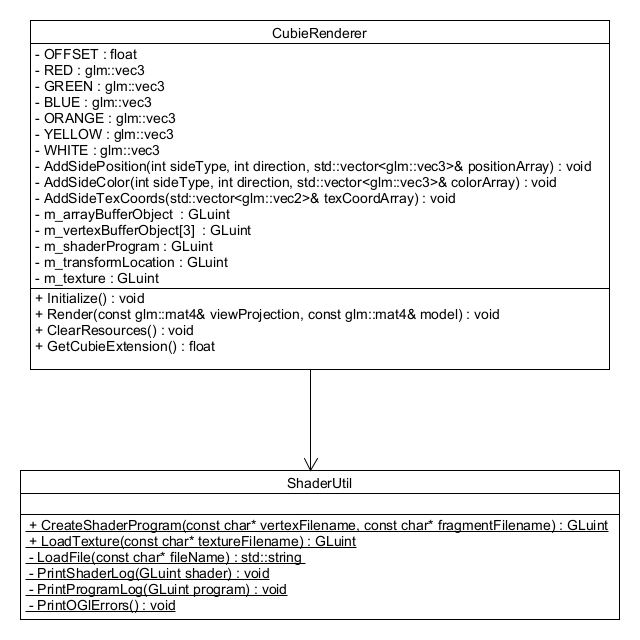
\includegraphics[scale=0.55]{images/CubieRendererClassDia.png}
	\caption{Klassendiagramm CubieRenderer und ShaderUtil}
	\label{CubieRendererDia}
\end{figure}

\section{RubiksCube und Cubie}
Die Klasse \texttt{RubiksCube} ist die zentrale Komponente des Spiels und implementiert die Logik für den Rubik's Cube. In der \texttt{Initialize(const RubiksGameInterface\& gameInterface)}-Methode wird die \texttt{CubieRenderer}-Instanz initialisiert, die für das Rendern der einzelnen Cubies verantwortlich ist. Zusätzlich wird ein dreidimensionales Gitter aus \texttt{Cubie}-Objekten erstellt. Jeder Cubie wird mit einer eindeutigen ID und einer Position im 3D-Raum initialisiert. Das \texttt{InputSystem}-Objekt wird aus dem übergebenen \texttt{RubiksGameInterface} extrahiert, um Benutzereingaben zu verarbeiten.

Ein \texttt{Cubie} ist ein einfaches Strukt, welches die Informationen über die Position, die sichtbare Rotation und die eingerastete Rotation eines Cubies speichert. Die sichtbare Rotation (\texttt{m\_visibleRotation}) wird für das Rendern verwendet, während die eingerastete Rotation (\texttt{m\_snapedRotation}) die korrekte Ausrichtung des Cubies im Gitter sicherstellt.

Die \texttt{Render(const glm::mat4\& viewProjection)}-Methode ist für die visuelle Darstellung des Rubik's Cube verantwortlich. Sie nutzt die übergebene View-Projection-Matrix, um sowohl die globale Rotation des gesamten Rubik's Cube als auch die individuelle Position jedes Cubies korrekt in der Szene darzustellen. Das \texttt{CubieRenderer}-Objekt rendert jeden Cubie einzeln unter Verwendung der entsprechenden Transformationsmatrizen.

Mit der \texttt{Update(const RubiksGameInterface\& gameInterface)}-Methode werden Benutzereingaben verarbeitet, insbesondere Mausinteraktionen. Außerdem aktualisiert sie die Snapping-Animation des Rubik's Cube. Durch die \texttt{UpdateMouse()}-Methode werden die Mausbewegungen und Klickzustände überwacht, um Aktionen wie das Drehen des gesamten Cubes oder einzelner Flächen einzuleiten. Beim Loslassen der linken Maustaste wird ein Soundeffekt abgespielt, um das Einrasten einer Fläche zu signalisieren.

Die Methode \texttt{DetermineClickedFace} identifiziert die angeklickte Fläche des Rubik's Cube, indem sie einen Strahl von der Mausposition in die Szene wirft und überprüft, welche Fläche geschnitten wird. Dabei durchläuft die Methode die Normalen der Flächen und nutzt das Skalarprodukt in Kombination mit der Funktion \texttt{glm::intersectRayPlane(...)}, um den Schnittpunkt zu bestimmen und die angeklickte Fläche zu identifizieren.

Die Methode \texttt{DetermineActiveSlice()} ist dafür verantwortlich, die zu drehende Fläche und Rotationschse des Rubik's Cube zu identifizieren, sobald der Spieler die linke Maustaste gedrückt hält und eine bestimmte Strecke auf dem Bildschirm zurücklegt (Dead Zone). 
Zunächst wird der Schnittpunkt zwischen dem Strahl, der beim Start des Ziehens erzeugt wurde, und der angeklickten Fläche des Rubik's Cube im Objektraum berechnet. Dieser Schnittpunkt dient als Basis, um die Slice-Indizes für die X-, Y- und Z-Achsen (\texttt{m\_xSliceIndex}, \texttt{m\_ySliceIndex} und \texttt{m\_zSliceIndex}) zu bestimmen. Diese Indizes geben an, in welchem Bereich des Rubik's Cube der Schnittpunkt liegt und welche Fläche gedreht werden soll.
Die Zugrichtung wird als die nächstgelegene Richtung zu den beiden verbleibenden orthogonalen Achsen bestimmt, die nicht der Normalen der angeklickten Fläche entsprechen.
Genau dafür ist die Methode \texttt{FindClosestDirection(const glm::vec3\& referenceDirection, const glm::vec3\& vecU, const glm::vec3\& vecV)} zu\-ständig. Sie berechnet das maximale Skalarprodukt zwischen der Zugrichtung und den beiden gegebenen Vektoren, die die orthogonalen Achsen repräsentieren. Anhand des Ergebnisses wird die aktive Drehachse (\texttt{m\_activeRotationAxis}) festgelegt.

\texttt{DeltaRotateSlice()} implementiert die Teilrotation einer Fläche des Rubik's Cube basierend auf der Mausbewegung. Die Methode wird aufgerufen, wenn der Spieler die linke Maustaste gedrückt hält und der Rubik's Cube sich im Rotationszustand befindet. Sie berechnet die Änderung der Bildschirmposition seit dem vorherigen Frame und verwendet diese, um die Rotationsstärke zu bestimmen.
Die Methode berechnet auch den gezogenen Vektor, der sich auf der Ebene der angeklickten Fläche befindet. Dieser Vektor wird dann auf einen weiteren Vektor projiziert, der orthogonal zu den Normalen der aktiven Drehachse und der angeklickten Fläche steht.
Die Methode berücksichtigt auch Sonderfälle, um sicherzustellen, dass die Rotation in die richtige Richtung erfolgt. Beispielsweise wird die Drehrichtung für bestimmte Flächen und Achsen umgekehrt, um die korrekte Ausrichtung zu gewährleisten. Dies geschieht durch die Überprüfung der aktuellen Fläche und der aktiven Drehachse.
Die berechnete Rotation wird dann auf jeden Cubie in der betroffenen Fläche angewendet. Dazu wird eine Rotationsmatrix erstellt, die die Drehung um die aktive Achse repräsentiert. Diese Matrix wird mit der sichtbaren Rotation jedes Cubies multipliziert, um die neue Ausrichtung zu berechnen.
Zusätzlich wird der Gesamtrotationsgrad der Fläche in der Variable \texttt{m\_totalFaceRotationDegree} gespeichert. Dieser Wert wird später verwendet, um die Einrast-Animation zu starten.

Wenn der Benutzer die Maustaste loslässt, die Einrast-Animation durchgeführt. Dafür ist die Methode \texttt{StartSnappingAnimation()} zuständig. Zuerst wird der Gesamtrotationsgrad auf [0, 360] normalisiert und auf die nächsten 90 Grad gerundet. Danach wird die Rotationsmatrix erstellt, die die Rotation der Fläche nach dem Einrasten darstellt. Diese Matrix wird dann auf jeden Cubie in der betroffenen Fläche angewendet. Die alten Rotationen werden für die kommende Interpolation gespeichert.

Die Methode \texttt{UpdateAnimation(float deltaTime)} aktualisiert die Einrast-Ani\-mation des Rubik's Cube basierend auf der vergangenen Zeit. 
Während der Animation wird eine sphärische lineare Interpolation (SLERP) verwendet, um die Rotationen der Cubies schrittweise zwischen ihrer alten und ihrer einrast Rotation zu interpolieren. Der \texttt{m\_tickCounter} wird basierend auf \texttt{deltaTime} erhöht, um den Fortschritt der Animation zu steuern. 
Wenn die Animation abgeschlossen ist (d.h., wenn der \texttt{m\_tickCounter} nahezu 1 erreicht), werden die sichtbaren Rotationen der Cubies auf ihre eingerasteten Rotationen gesetzt, und das 3D-Gitter wird entsprechend der Anzahl der Drehungen aktualisiert. Dies geschieht durch Transponieren und Invertieren der betroffenen Fläche.
Zum Schluss werden alle relevanten Variablen zurückgesetzt, und der Zustand des Cubes wird auf \texttt{AnimationState::STABLE} gesetzt.

Die Methode \texttt{ForEachInSlice(Func func)} ist eine  template-Funktion, die eine übergebene Funktion auf alle Cubies in der aktiven Fläche anwendet. Diese Methode ermöglicht eine effiziente Iteration durch die Cubies im aktuellen Slice und vermeidet die Speicherung zusätzlicher Teilmengen des Gitters.

Die \texttt{ClearResources()}-Methode gibt alle Ressourcen des Rubik's Cube frei, einschließlich der Freigabe des \texttt{CubieRenderer}-Objekts und des Löschens aller \texttt{Cubie}-Pointer im 3D-Gitter.

Eine detaillierte Übersicht der Klassenstruktur und der Beziehungen zwischen den Komponenten ist in Abbildung \ref{RubiksCubeClassDia} dargestellt.

\begin{figure} [H]
	\centering
	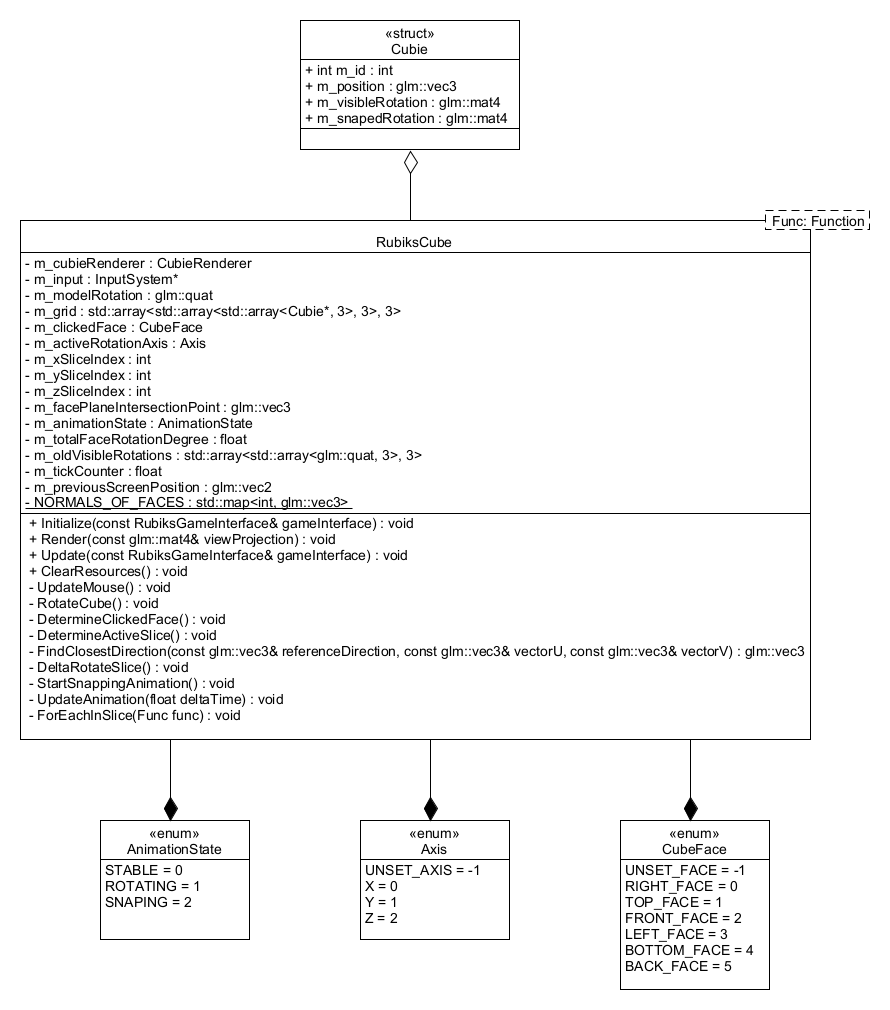
\includegraphics[scale=0.475]{images/RubiksCubeClassDia.png}
	\caption{Klassendiagramm RubiksCube und Cubie}
	\label{RubiksCubeClassDia}
\end{figure}


%------------------ Literaturverzeichnis & Index -------------------------------
\backmatter
%\bibliography{literatur}								% Literaturverzeichnis (literatur.bib)
%\printindex												% Index (optional)


%------------------ Anhänge ----------------------------------------------------
\begin{appendix}
	%\chapter{Glossar}

\abbreviation{DisASTer}		{Distributed Algorithms Simulation Terrain, eine Plattform zur Implementierung verteilter Algorithmen \cite{Gottwald:03}}

\abbreviation{DSM}			{Distributed Shared Memory}

\abbreviation{AC}			{Atomic Consistency (dt.: Linearisierbarkeit)}
\abbreviation{RC}			{Release Consistency (dt.: Freigabekonsistenz)}
\abbreviation{SC}			{Sequential Consistency (dt.: Sequentielle Konsistenz)}
\abbreviation{WC}			{Weak Consistency (dt.: Schwache Konsistenz)}
							% Glossar (optional)
	%\chapter{Selbstständigkeitserklärung}

\begin{description}

\item[$\Box$] Diese Arbeit habe ich selbstständig verfasst und keine anderen als die angegebenen Quellen und Hilfsmittel verwendet.\\

\item[$\Box$] Diese Arbeit wurde als Gruppenarbeit angefertigt. Meinen Anteil habe ich selbstständig verfasst und keine anderen als die angegebenen Quellen und Hilfsmittel verwendet.\\

Namen der Mitverfasser:
\vspace{3cm}

Meine eigene Leistung ist:
\vspace{3cm}

\end{description}

\vspace{3cm}

\begin{minipage}[t]{3cm}
	\rule{3cm}{0.5pt}
	Datum
\end{minipage}
\hfill
\begin{minipage}[t]{9cm}
	\rule{9cm}{0.5pt}
	Unterschrift der Kandidatin/des Kandidaten
\end{minipage}
	% Selbstständigkeitserklärung
\end{appendix}


\end{document}
